\subsection{Sin pérdida de paquetes ($p$ = 0)}

\subsubsection{Sin varianza}

\begin{figure}[H]
\begin{minipage}{0.5\linewidth}
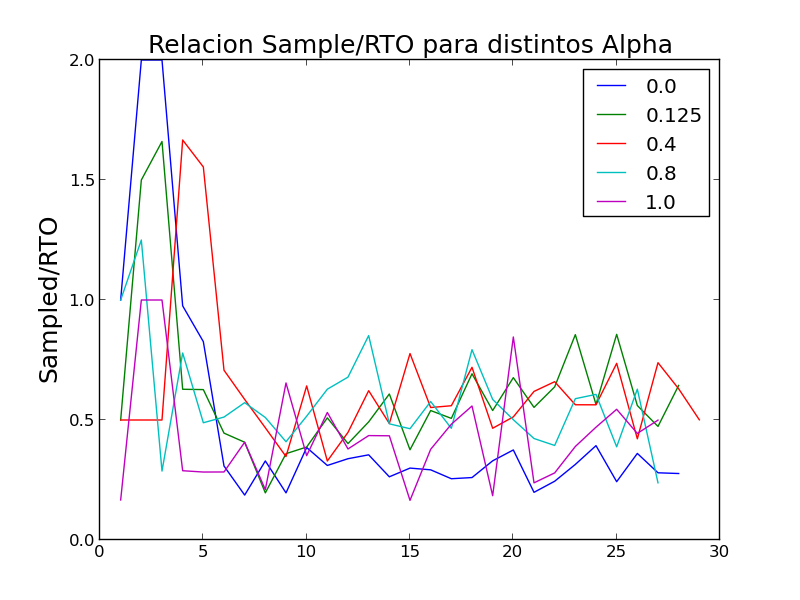
\includegraphics[width=\linewidth]{../graficos/alphavar0drop0.png}
\caption{Relación Sample/RTO, $\beta$ = 0.25}\label{fig:alpha-var0-drop0}
\end{minipage}
\hfill
\begin{minipage}{0.5\linewidth}
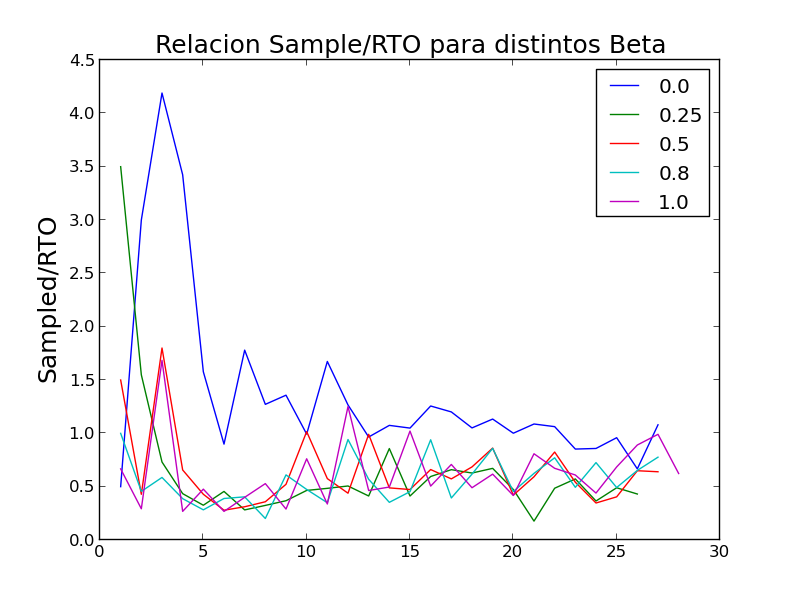
\includegraphics[width=\linewidth]{../graficos/betavar0drop0.png}
\caption{Relación Sample/RTO, $\alpha$ = 0.125}\label{fig:beta-var0-drop0}
\end{minipage}
\end{figure}

\subsubsection{Varianza media}

\begin{figure}[H]
\begin{minipage}{0.5\linewidth}
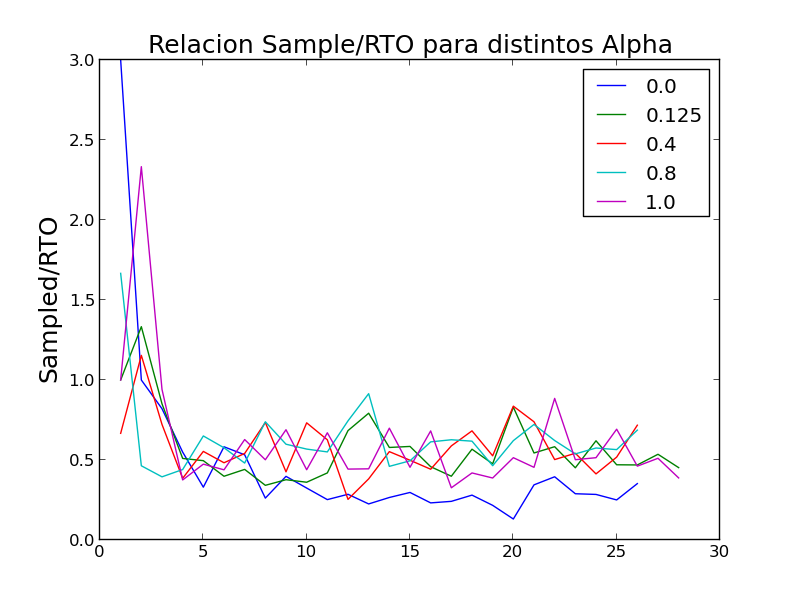
\includegraphics[width=\linewidth]{../graficos/alphavar2drop0.png}
\caption{Relación Sample/RTO, $\beta$ = 0.25}\label{fig:alpha-var2-drop0}
\end{minipage}
\hfill
\begin{minipage}{0.5\linewidth}
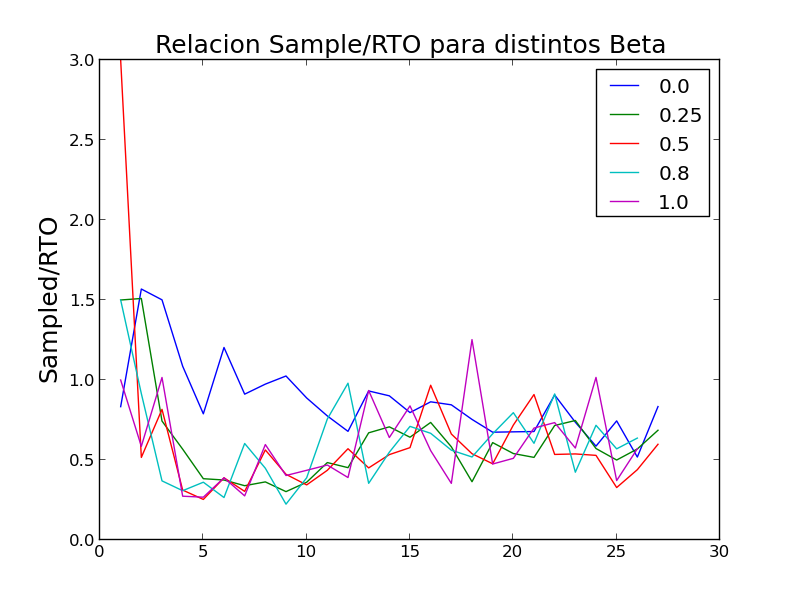
\includegraphics[width=\linewidth]{../graficos/betavar2drop0.png}
\caption{Relación Sample/RTO, $\alpha$ = 0.125}\label{fig:beta-var2-drop0}
\end{minipage}
\end{figure}

\subsubsection{Varianza alta}

\begin{figure}[H]
\begin{minipage}{0.5\linewidth}
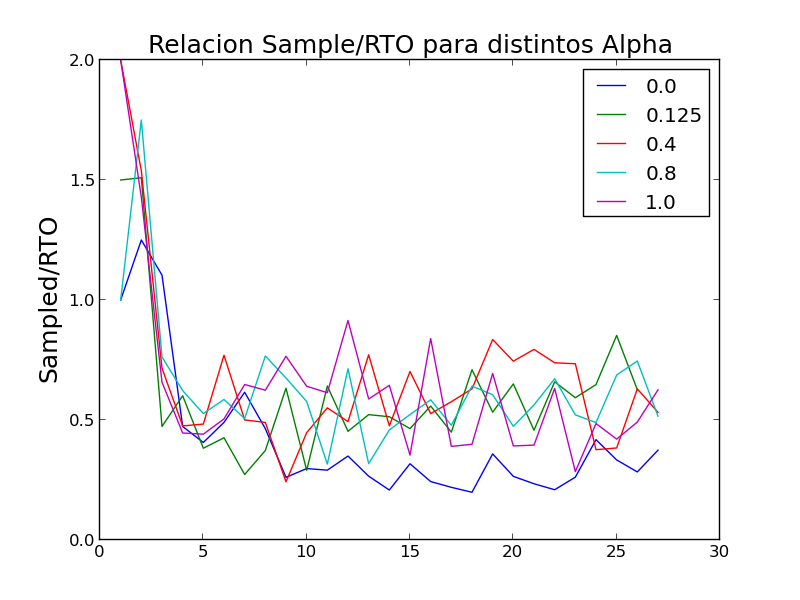
\includegraphics[width=\linewidth]{../graficos/alphavar5drop0.png}
\caption{Relación Sample/RTO, $\beta$ = 0.25}\label{fig:alpha-var5-drop0}
\end{minipage}
\hfill
\begin{minipage}{0.5\linewidth}
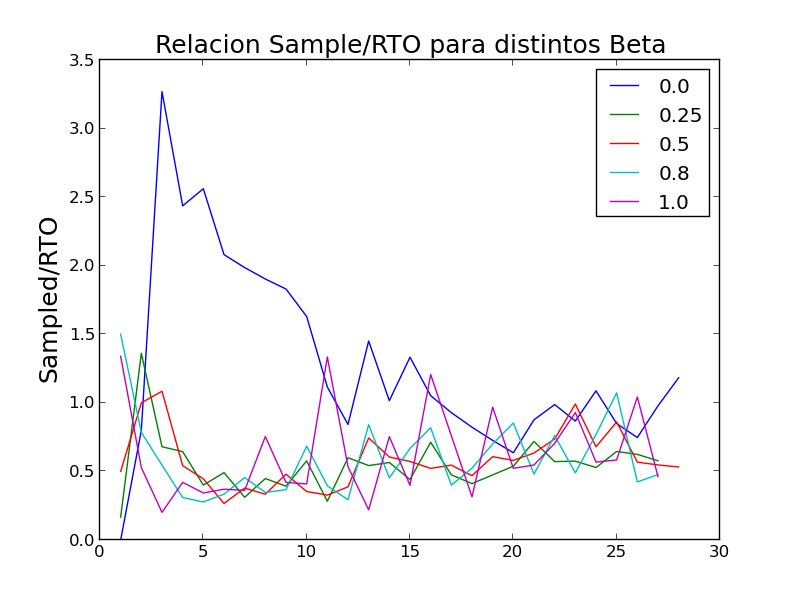
\includegraphics[width=\linewidth]{../graficos/betavar5drop0.png}
\caption{Relación Sample/RTO, $\alpha$ = 0.125}\label{fig:beta-var5-drop0}
\end{minipage}
\end{figure}


\subsection{Pérdida de paquetes baja ($p$ = 0,30)}
\subsubsection{Sin varianza}

\begin{figure}[H]
\begin{minipage}{0.5\linewidth}
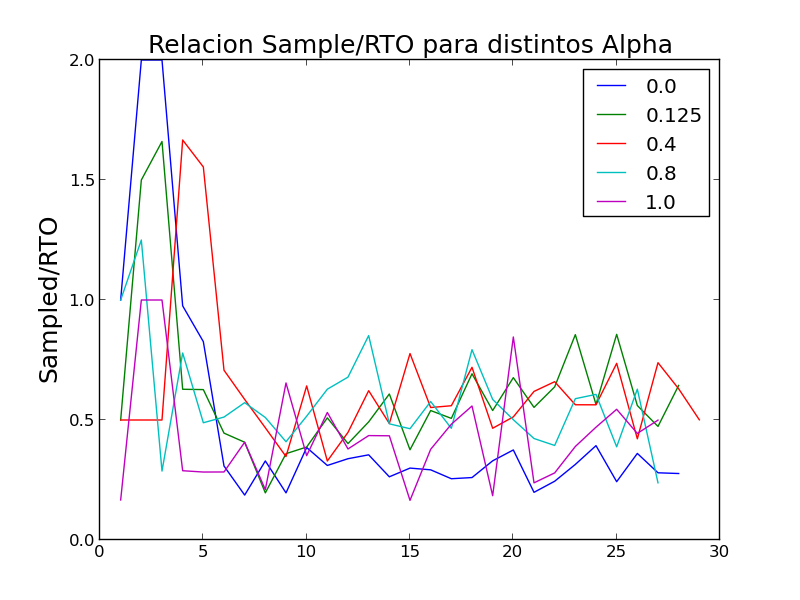
\includegraphics[width=\linewidth]{../graficos/alphavar0drop30.png}
\caption{Relación Sample/RTO, $\beta$ = 0.25}\label{fig:alpha-var0-drop30}
\end{minipage}
\hfill
\begin{minipage}{0.5\linewidth}
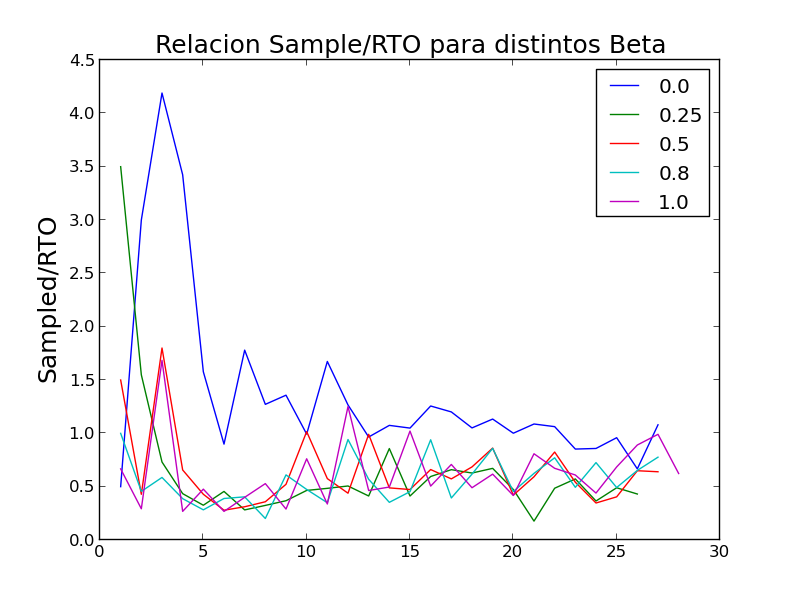
\includegraphics[width=\linewidth]{../graficos/betavar0drop30.png}
\caption{Relación Sample/RTO, $\alpha$ = 0.125}\label{fig:beta-var0-drop30}
\end{minipage}
\end{figure}

\subsubsection{Varianza media}

\begin{figure}[H]
\begin{minipage}{0.5\linewidth}
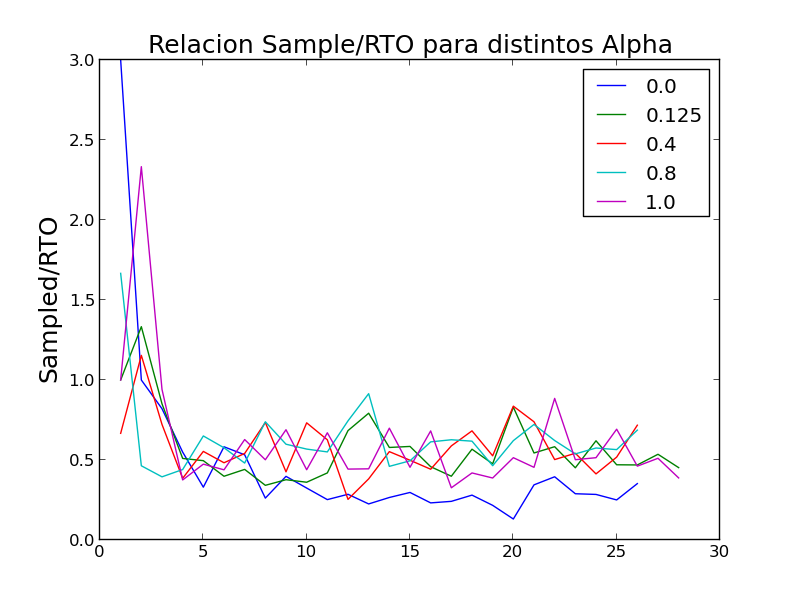
\includegraphics[width=\linewidth]{../graficos/alphavar2drop30.png}
\caption{Relación Sample/RTO, $\beta$ = 0.25}\label{fig:alpha-var2-drop30}
\end{minipage}
\hfill
\begin{minipage}{0.5\linewidth}
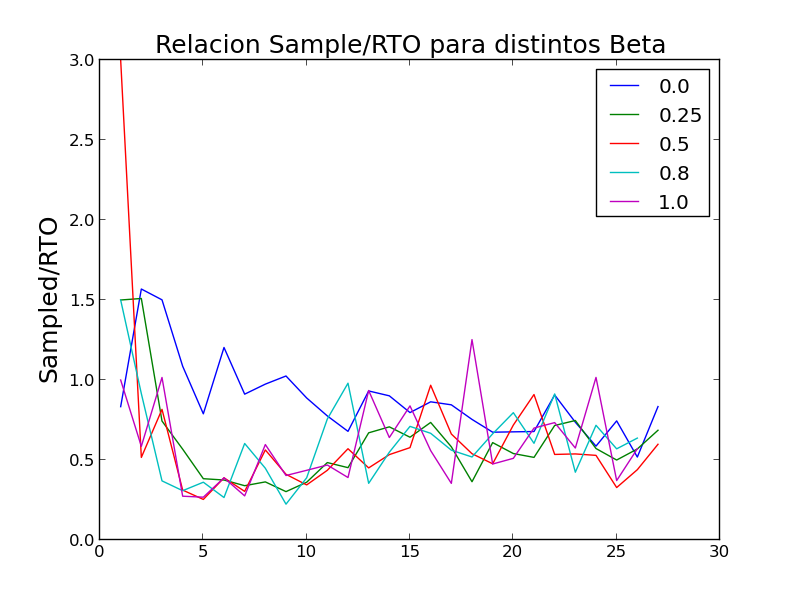
\includegraphics[width=\linewidth]{../graficos/betavar2drop30.png}
\caption{Relación Sample/RTO, $\alpha$ = 0.125}\label{fig:beta-var2-drop30}
\end{minipage}
\end{figure}

\subsubsection{Varianza alta}

\begin{figure}[H]
\begin{minipage}{0.5\linewidth}
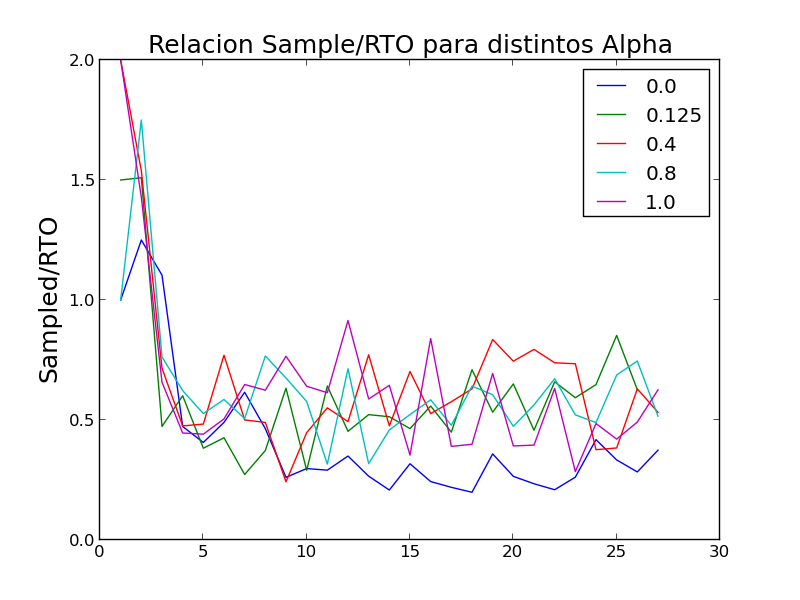
\includegraphics[width=\linewidth]{../graficos/alphavar5drop30.png}
\caption{Relación Sample/RTO, $\beta$ = 0.25}\label{fig:alpha-var5-drop30}
\end{minipage}
\hfill
\begin{minipage}{0.5\linewidth}
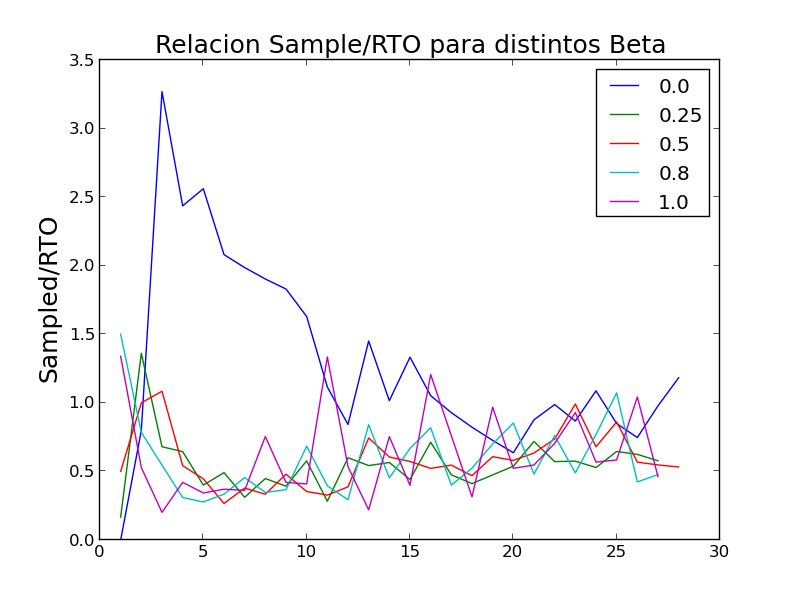
\includegraphics[width=\linewidth]{../graficos/betavar5drop30.png}
\caption{Relación Sample/RTO, $\alpha$ = 0.125}\label{fig:beta-var5-drop30}
\end{minipage}
\end{figure}

\subsection{Pérdida de paquetes alta ($p$ = 0,7)}
\subsubsection{Sin varianza}

\begin{figure}[H]
\begin{minipage}{0.5\linewidth}
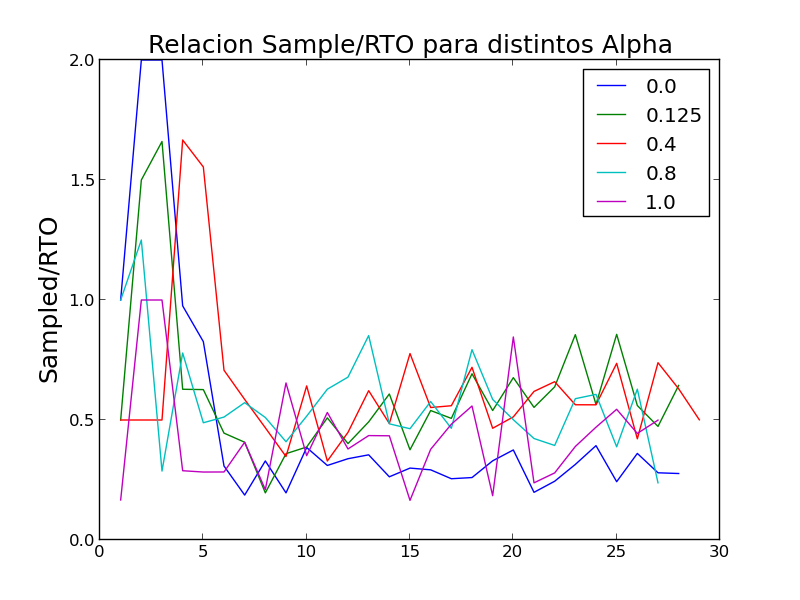
\includegraphics[width=\linewidth]{../graficos/alphavar0drop70.png}
\caption{Relación Sample/RTO, $\beta$ = 0.25}\label{fig:alpha-var0-drop70}
\end{minipage}
\hfill
\begin{minipage}{0.5\linewidth}
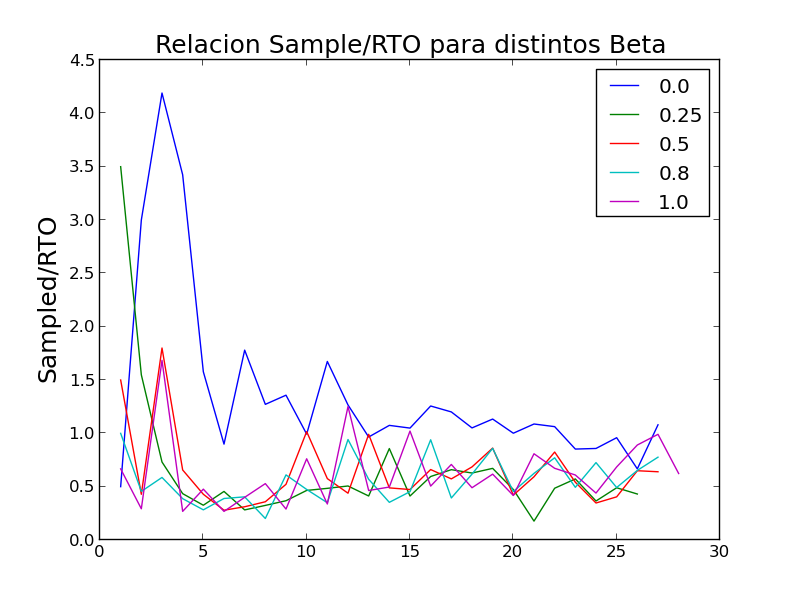
\includegraphics[width=\linewidth]{../graficos/betavar0drop70.png}
\caption{Relación Sample/RTO, $\alpha$ = 0.125}\label{fig:beta-var0-drop70}
\end{minipage}
\end{figure}

\subsubsection{Varianza media}

\begin{figure}[H]
\begin{minipage}{0.5\linewidth}
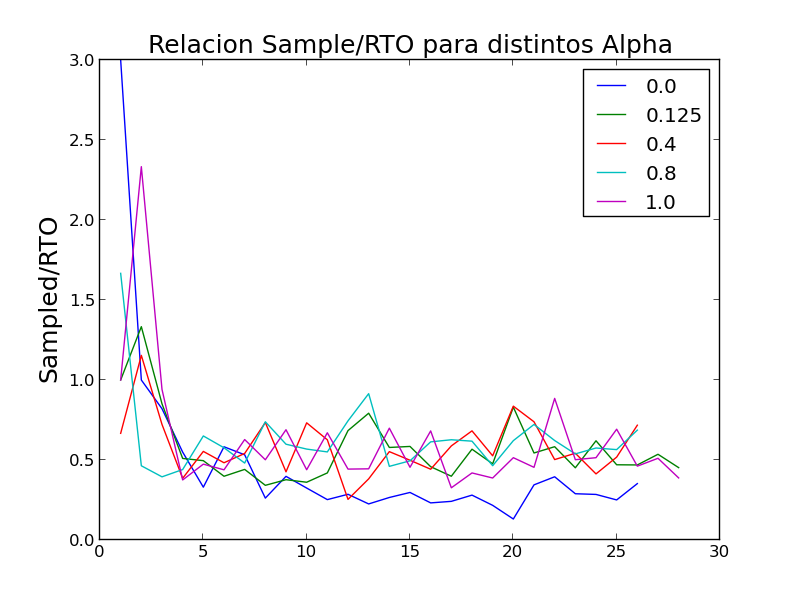
\includegraphics[width=\linewidth]{../graficos/alphavar2drop70.png}
\caption{Relación Sample/RTO, $\beta$ = 0.25}\label{fig:alpha-var2-drop70}
\end{minipage}
\hfill
\begin{minipage}{0.5\linewidth}
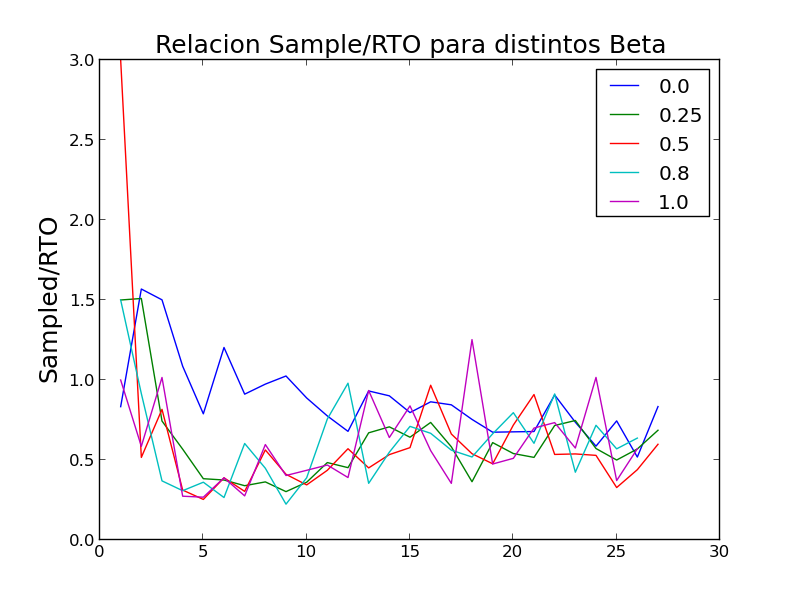
\includegraphics[width=\linewidth]{../graficos/betavar2drop70.png}
\caption{Relación Sample/RTO, $\alpha$ = 0.125}\label{fig:beta-var2-drop70}
\end{minipage}
\end{figure}

\subsubsection{Varianza alta}

\begin{figure}[H]
\begin{minipage}{0.5\linewidth}
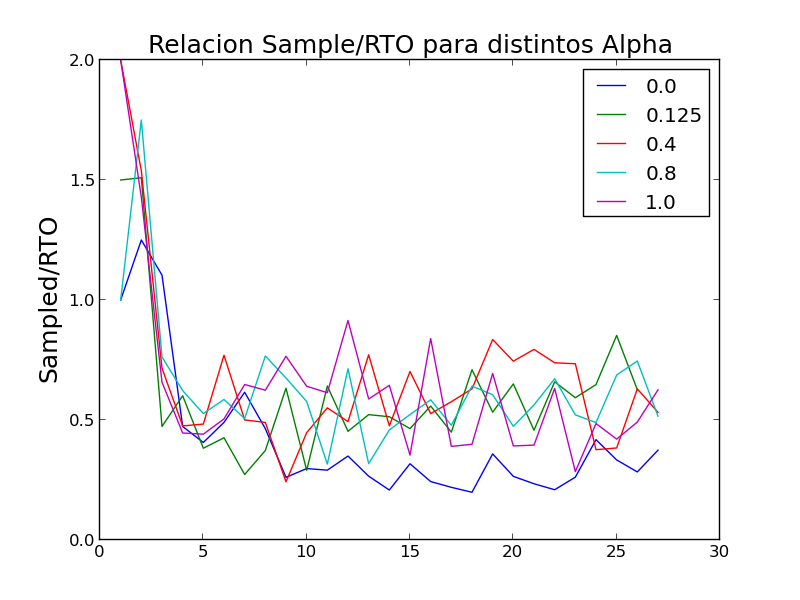
\includegraphics[width=\linewidth]{../graficos/alphavar5drop70.png}
\caption{Relación Sample/RTO, $\beta$ = 0.25}\label{fig:alpha-var5-drop70}
\end{minipage}
\hfill
\begin{minipage}{0.5\linewidth}
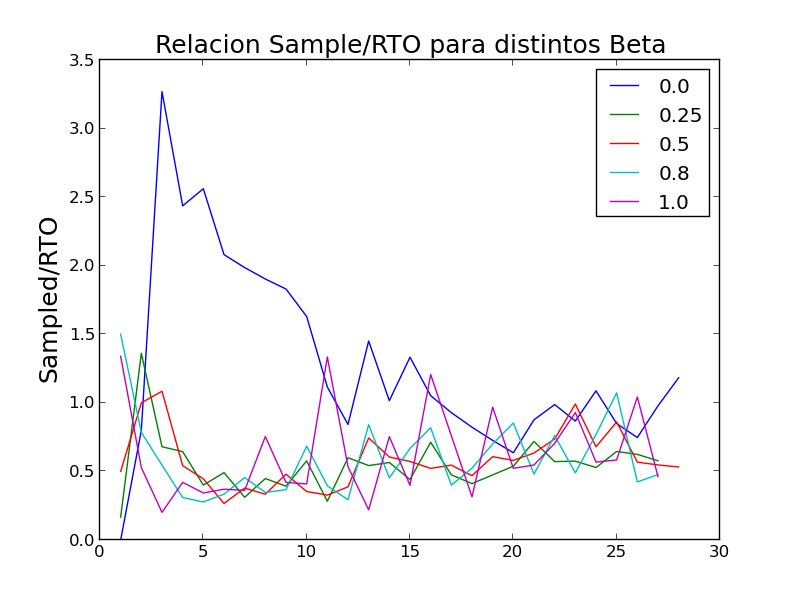
\includegraphics[width=\linewidth]{../graficos/betavar5drop70.png}
\caption{Relación Sample/RTO, $\alpha$ = 0.125}\label{fig:beta-var5-drop70}
\end{minipage}
\end{figure}